% Sección del informe de la Entrega 3: índices espaciales y análisis exploratorio de los edificios.
\section{Índices Espaciales y Análisis Exploratorio}

\subsection{Índices y evidencia}
Cada colección tiene tres índices creados por \texttt{src/02\_load\_buildings.py}. El índice \texttt{geometry\_2dsphere} permite consultas con \texttt{\$geoIntersects}, \texttt{\$geoWithin} y \texttt{\$near}. El índice compuesto sobre \texttt{(municipality\_code, area\_m2)} permite buscar los techos de un municipio y ordenarlos por área. El índice \texttt{source\_file} facilita localizar los documentos por partición de origen. \texttt{buildings\_google} también tiene un índice sobre \texttt{confidence}.

\begin{table}[H]
\centering
\footnotesize
\resizebox{\linewidth}{!}{\begin{tabular}{p{0.2\linewidth}p{0.2\linewidth}p{0.17\linewidth}rrr}
\toprule
Colección & Consulta & Plan & Docs (índice) & Docs (sin índice) & ms \\
\midrule
\texttt{buildings\_microsoft} & \texttt{punto\_en\_edificio} & FETCH/IXSCAN & 5 & 1761043 & 2 \\
\texttt{buildings\_microsoft} & \texttt{cercanos\_near} & GEO\_NEAR\_2DSPHERE/FETCH/IXSCAN/FETCH/IXSCAN & 1191 & -- & 10 \\
\texttt{buildings\_google} & \texttt{punto\_en\_edificio} & FETCH/IXSCAN & 8 & 2694782 & 2 \\
\texttt{buildings\_google} & \texttt{cercanos\_near} & GEO\_NEAR\_2DSPHERE/FETCH/IXSCAN/FETCH/IXSCAN & 813 & -- & 14 \\
\bottomrule
\end{tabular}
}
\caption{Planes de ejecución con índice y con recorrido completo.}
\label{tab:evidencia_edificios}
\end{table}

En la consulta de intersección de un punto, \texttt{explain("executionStats")} mostró \texttt{FETCH/IXSCAN}. MongoDB examinó 5 documentos de Microsoft y 8 de Google con el índice. Con \texttt{COLLSCAN}, examinó 1.761.043 y 2.694.782 documentos, respectivamente, y devolvió la misma huella de cada fuente. En Sipí (27745), la validación cruzada entre la asignación por código y \texttt{\$geoWithin} dio 651 de 653 huellas para Microsoft (99,7\,\%) y 1 de 1 para Google (100\,\%). Ambas cifras superaron el umbral del 95\,\% en el municipio evaluado.

\subsection{Análisis exploratorio}
El análisis usa agregaciones de MongoDB. El criterio de techo apto, parametrizado en \texttt{config/params.yaml}, requiere una huella de al menos 15\,m$^2$ y, para Google, confianza de al menos 0,70.

\begin{table}[H]
\centering
\footnotesize
\resizebox{\linewidth}{!}{\begin{tabular}{lrrrrrrr}
\toprule
Fuente & Edificios & Área media (m\textsuperscript{2}) & Mediana (m\textsuperscript{2}) & P99 (m\textsuperscript{2}) & Área total (km\textsuperscript{2}) & Techos aptos & Área apta (km\textsuperscript{2}) \\
\midrule
microsoft & 1,761,043 & 125.6 & 77.0 & 912.5 & 221.13 & 1,756,529 & 221.07 \\
google & 2,694,782 & 82.8 & 58.1 & 446.9 & 223.01 & 2,161,261 & 206.28 \\
\bottomrule
\end{tabular}
}
\caption{Resumen de huellas y techos aptos por fuente.}
\end{table}

\begin{figure}[H]
\centering
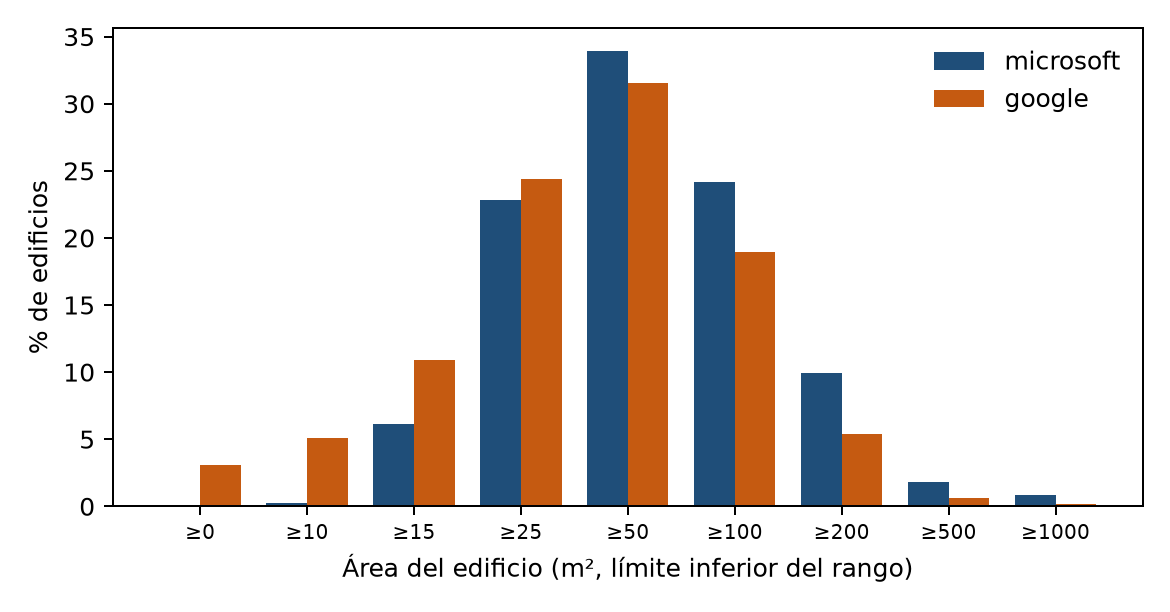
\includegraphics[width=0.85\linewidth]{../eda/hist_area.png}
\caption{Distribución del área de las huellas por fuente.}
\end{figure}

\begin{itemize}
  \item \textbf{Conteo y área.} Microsoft registró 1.761.043 huellas en 170 municipios PDET y Google, 2.694.782 en 165. Google aportó 933.739 huellas más (53,0\,\%), con una mediana de área menor (58,1 frente a 77,0\,m$^2$). Las áreas totales fueron similares (223,01\,km$^2$ en Google y 221,13\,km$^2$ en Microsoft).
  \item \textbf{Cobertura.} Google no registró huellas en Murindó, Vigía del Fuerte, Bojayá, Medio San Juan ni Nóvita. Estos casos corresponden a ausencia de datos de Google.
  \item \textbf{Área de Google.} El área original \texttt{area\_in\_meters} es en promedio 0,37\,\% inferior al área recalculada en EPSG:9377. El análisis usa el valor original de Google para aplicar el umbral de área.
  \item \textbf{Confianza.} Los intervalos de mayor frecuencia fueron $[0{,}75;0{,}80)$ y $[0{,}80;0{,}85)$, que concentran el 47,6\,\% de las huellas de Google. De las 2.476.119 huellas que cumplen el área mínima, el umbral de 0,70 excluyó 314.858 (12,7\,\%). Quedaron 2.161.261 techos aptos en Google y 1.756.529 en Microsoft, con 206,28 y 221,07\,km$^2$ de área apta, respectivamente.
  \item \textbf{Municipios con más techos aptos.} Santa Marta lideró en ambas fuentes (67.486 en Microsoft y 147.798 en Google), seguida de Valledupar (63.556 y 134.865, respectivamente). Turbo fue tercero por conteo en Microsoft (43.199) y Buenaventura en Google (85.643). Por área apta, Santa Marta, Valledupar y Buenaventura ocuparon los tres primeros lugares en ambas fuentes.
  \item \textbf{Solapamiento.} De 500 huellas de Google elegidas al azar entre las de al menos 15\,m$^2$, 356 (71,2\,\%) intersectaron al menos una huella de Microsoft. El porcentaje mide intersección geométrica en esa muestra.
\end{itemize}
